% !TeX spellcheck = en_GB
\chapter{Methods}
\label{ch:methods}
First, we evaluated the \textit{VL53L0X ToF Ranging Sensor} with a \textit{mbed LPC1768} microcontroller on its potential use for obstacle avoidance on a MAV (\cref{sec:tof}). Second, we integrated the sensors on the pixhawk autopilot (\cref{sec:pixhawk}). Last, we implemented a potential field in the pixhawk (\cref{sec:potential field}). 

\section{Time-of-Flight Ranging Sensor}
\label{sec:tof}
For this thesis we've decided on using the \textit{VL53L0X ToF Ranging Sensor} developed by \textit{STMicroelectronics} for the distance measurements. For the evaluation we connected the sensor via I2C to a \textit{mbed LPC1768} microcontroller. The sensor has a range of \unit[0]{mm} up to \unit[2]{m} under optimal conditions, i.e. no infrared radiation. The sensor allows four different modes to be used (\cref{tab:profile}). To facilitate the integration we use a satellite board. The VL53L0X sensor comes with a Application Programming Interface (API) which allows to control of the VL53L0X Firmware like initialisation/calibration, ranging Start/Stop, choice of accuracy and choice of ranging mode.

\begin{table}[]
	\centering
	\caption{Range profile}
	\label{tab:profile}
	\resizebox{\textwidth}{!}{%
		\begin{tabular}{|c|c|c|c|}
			\hline
			\textbf{Range Profile} & \textbf{Range Timing Budget} & \textbf{Typical Performance} & \textbf{Typical Application}                                                             \\ 
			\specialrule{.2em}{.1em}{.1em} 
			Default Mode           & 30 ms                        & 1.2 m                        & Standard                                                                                 \\ \hline
			High Accuracy          & 200 ms                       & 1.2 m                        & Precise Measurement                                                                      \\ \hline
			Long Range             & 33 ms                        & 2 m                          & \begin{tabular}[c]{@{}c@{}}Long Rangin,\\  only for dark conditions (no IR)\end{tabular} \\ \hline
			High Speed             & 20 ms                        & 1.2 m                        & \begin{tabular}[c]{@{}c@{}}High Speed, \\ where accuracy is not important\end{tabular}   \\ \hline
		\end{tabular}%
	}
\end{table}


\subsection{Evaluation}
\label{subs:evaluation}
We evaluated the sensor's performance using different target surfaces and under different lightning conditions. During the measurements we changed the angles and distance relative to the target. For the ground truth measurement we used a yardstick and a protractor. We conducted 100 measurements for every measurement setup.\\
The surfaces used for the evaluation were a white plastered wall, a concrete wall and a wooden wall (\cref{fig:surfaces}). We have chosen these surfaces, since most walls inside of a building consist of these materials. The experiments were conducted inside. The results of the measurements using different surface did not show a significant difference between the surfaces (\crefrange{fig:surface_hist_con}{fig:surface_hist_white}). 
\begin{figure}
	\centering
	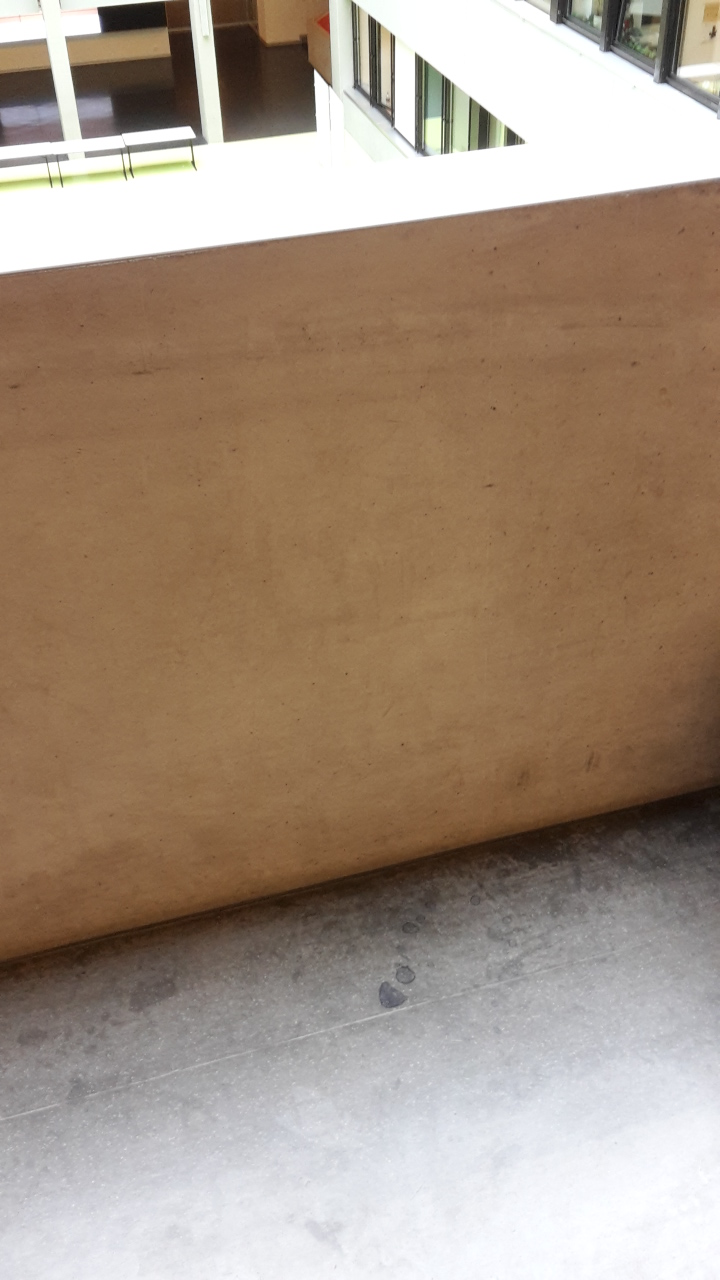
\includegraphics[width=.3\linewidth]{pictures/concrete_wall.jpg}\quad
	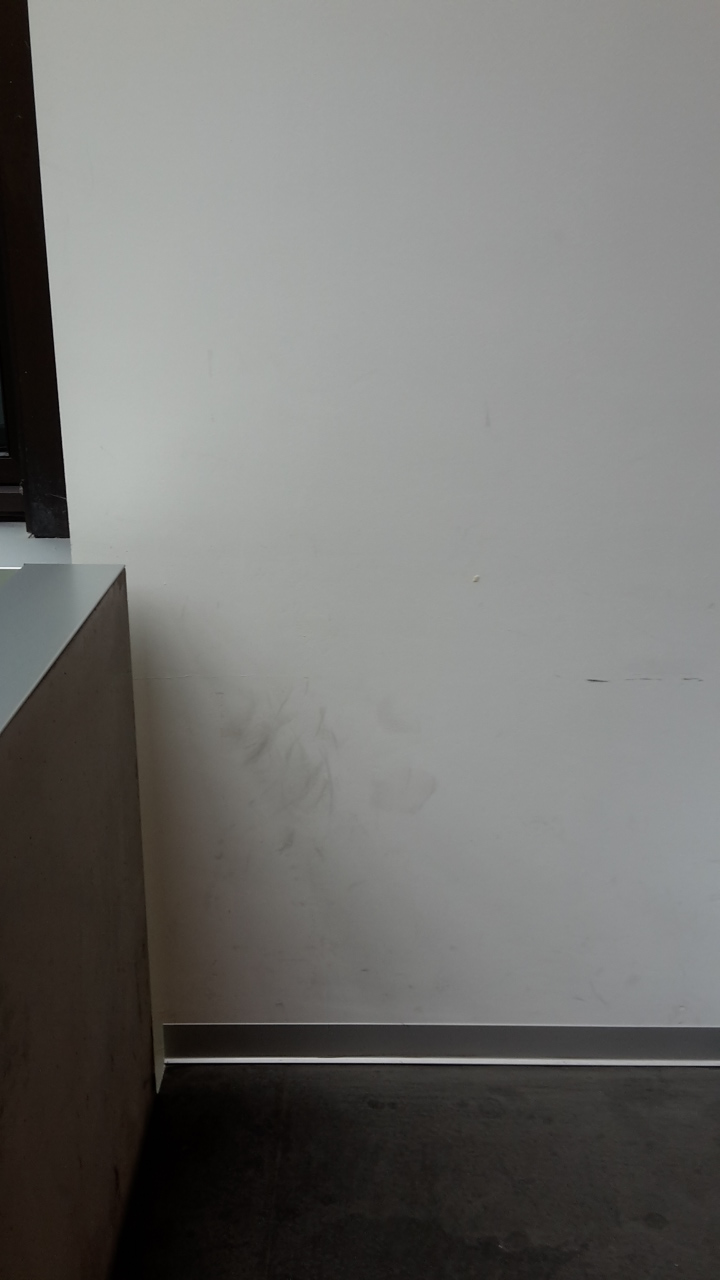
\includegraphics[width=.3\linewidth]{pictures/white_wall.jpg}\quad
	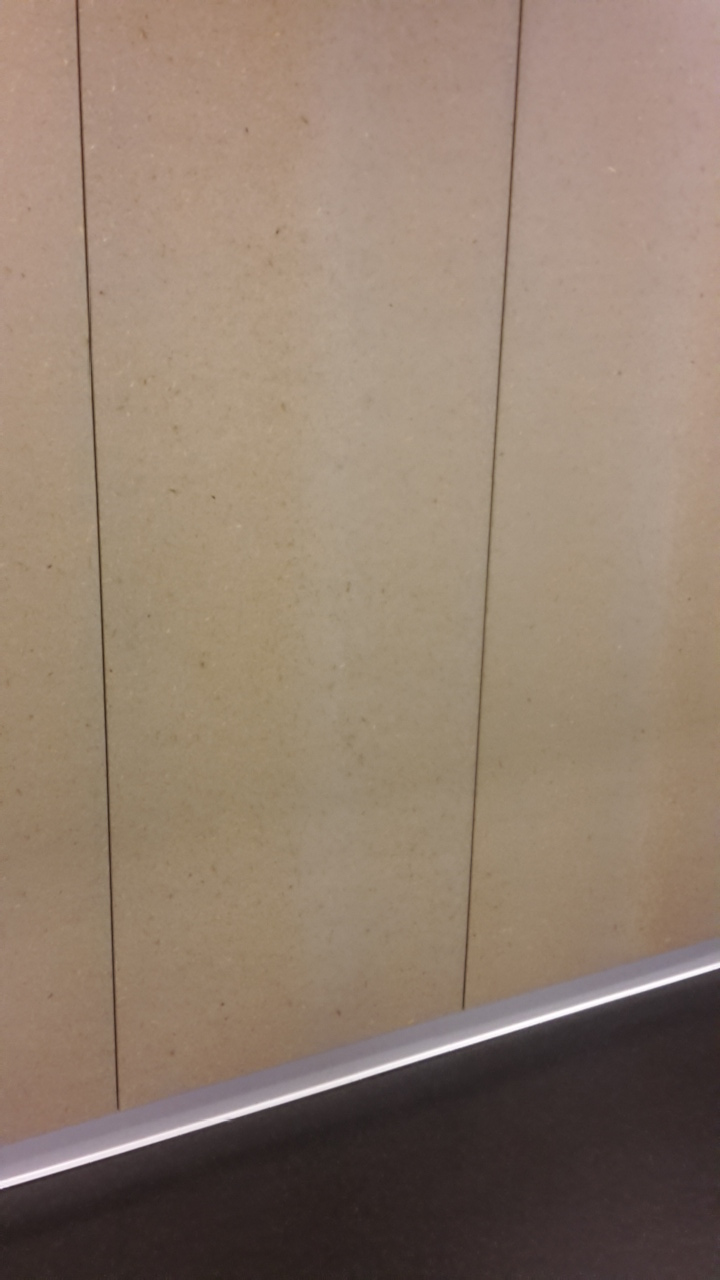
\includegraphics[width=.3\linewidth]{pictures/wooden_wall.jpg}
	\caption{Different surfaces used for the evaluation.}
	\label{fig:surfaces}
\end{figure}

\begin{figure}
	\centering
	\begin{minipage}{0.3\textwidth}
		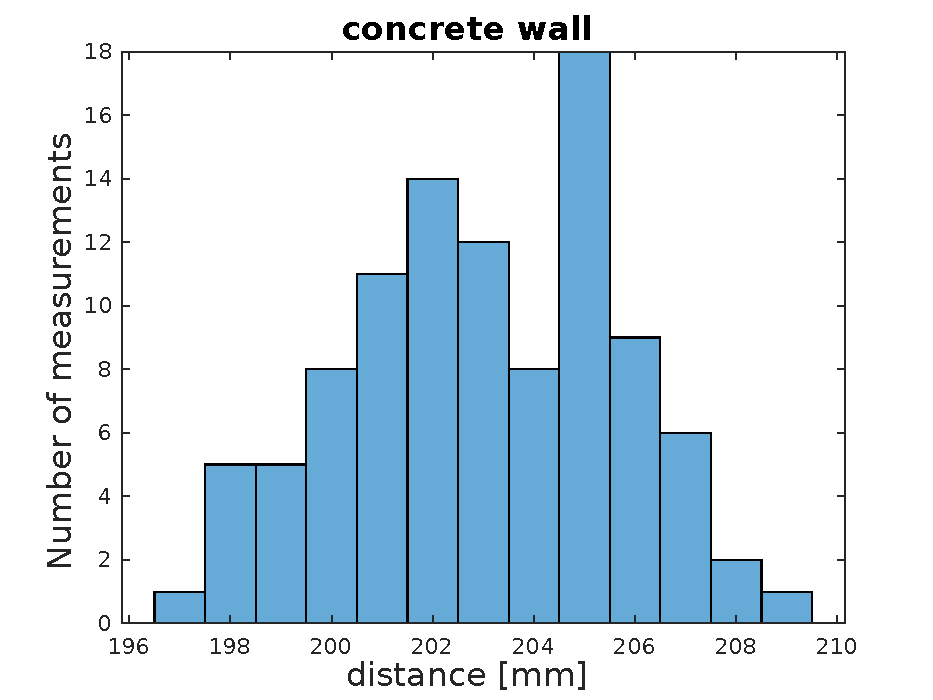
\includegraphics[width=0.9\linewidth]{pictures/concrete_hist.pdf}
		\caption{ground truth distance $d_{truth}= \unit[20]{mm}$, Standard Error: $\sigma=\unit[2.03]{mm}$, Expected Value: $E=\unit[203]{mm}$}
		\label{fig:surface_hist_con}
	\end{minipage}
	\quad
	\begin{minipage}{0.3\textwidth}
		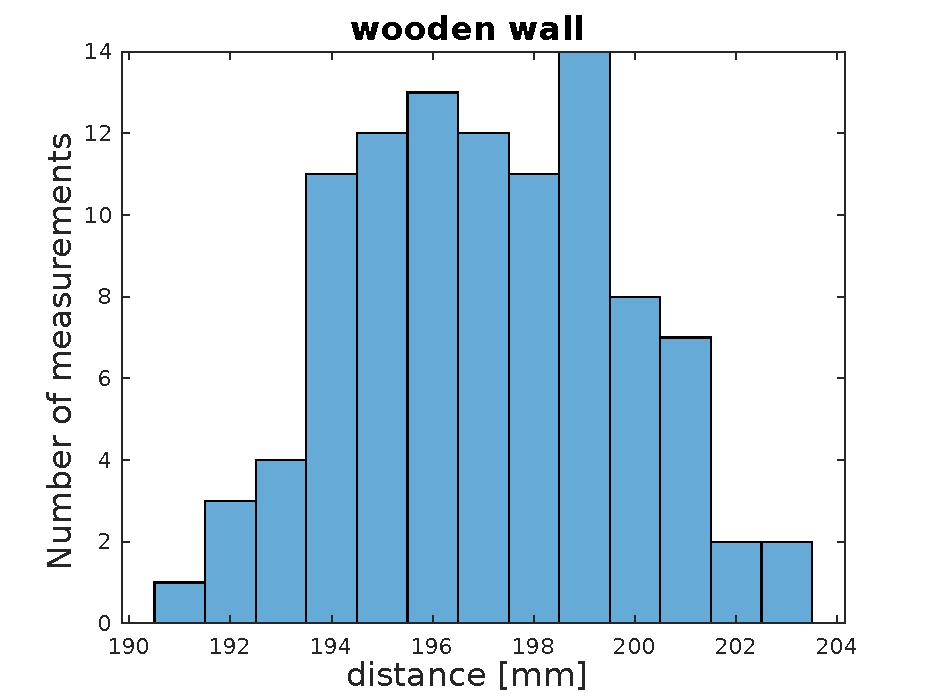
\includegraphics[width=0.9\linewidth]{pictures/wooden_wall.pdf}
		\caption{ground truth distance $d_{truth}= \unit[20]{mm}$, Standard Error: $\sigma=\unit[2.67]{mm}$, Expected Value: $E=\unit[197.06]{mm}$}
		\label{fig:surface_hist_wood}
	\end{minipage}
	\quad
	\begin{minipage}{0.3\textwidth}
		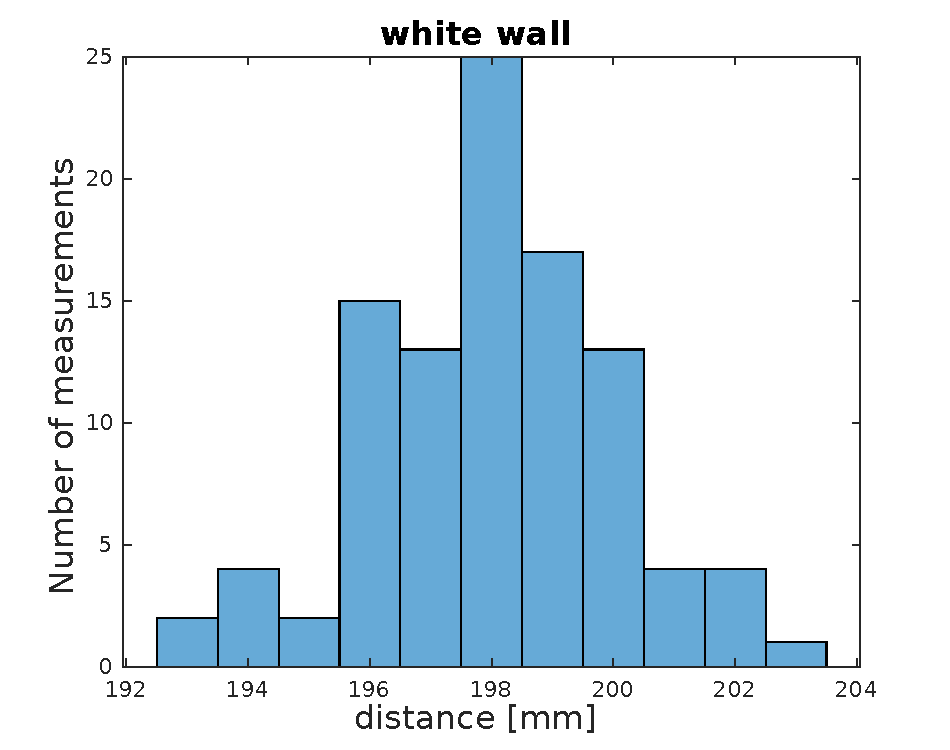
\includegraphics[width=0.9\linewidth]{pictures/white_wall.pdf}
		\caption{ground truth distance $d_{truth}= \unit[20]{mm}$, Standard Error: $\sigma=\unit[2.01]{mm}$, Expected Value: $E=\unit[198.01]{mm}$}
		\label{fig:surface_hist_white}
	\end{minipage}
\end{figure}

Increasing the angle sharpness or the distance of the sensor relative to the wall does not significantly affect the accuracy of the sensor (\crefrange{fig:angle90}{fig:angl22.5}).\\

\begin{figure}
	\centering
	\begin{minipage}{0.3\textwidth}
		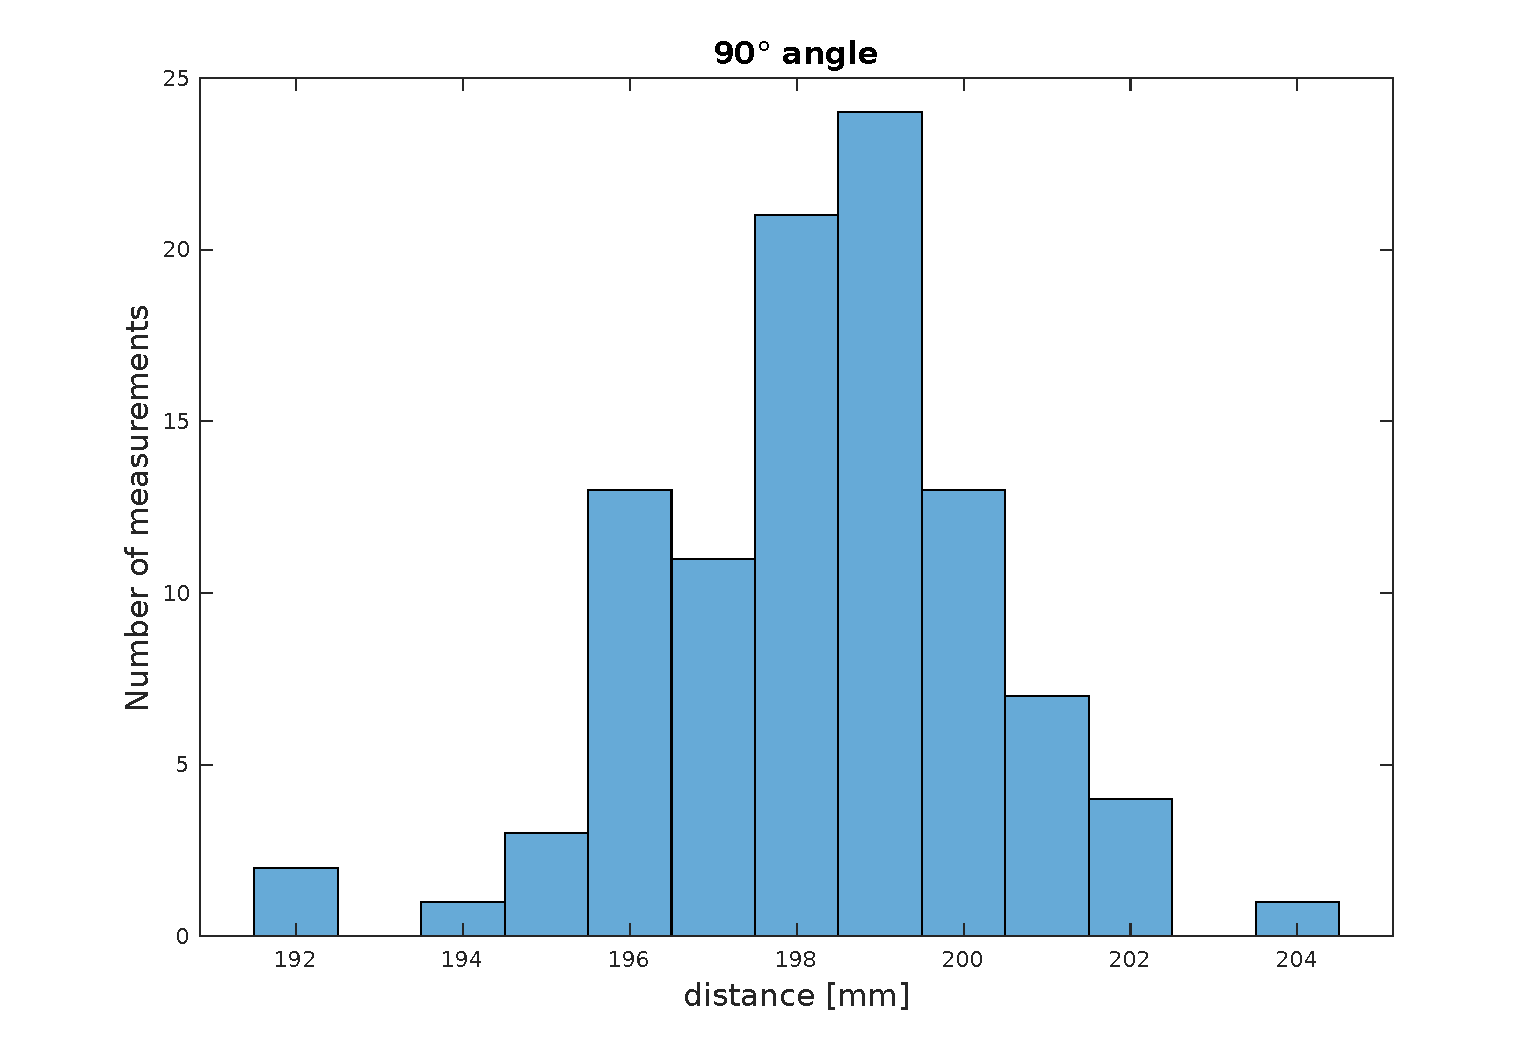
\includegraphics[width=0.9\linewidth]{pictures/plot_angles_90.pdf}
		\caption{ground truth distance $d_{truth}= \unit[20]{mm}$, Standard Error: $\sigma=\unit[2.03]{mm}$, Expected Value: $E=\unit[198.31]{mm}$, Relative angle: 90°}
		\label{fig:angle90}
	\end{minipage}
	\quad
	\begin{minipage}{0.3\textwidth}
		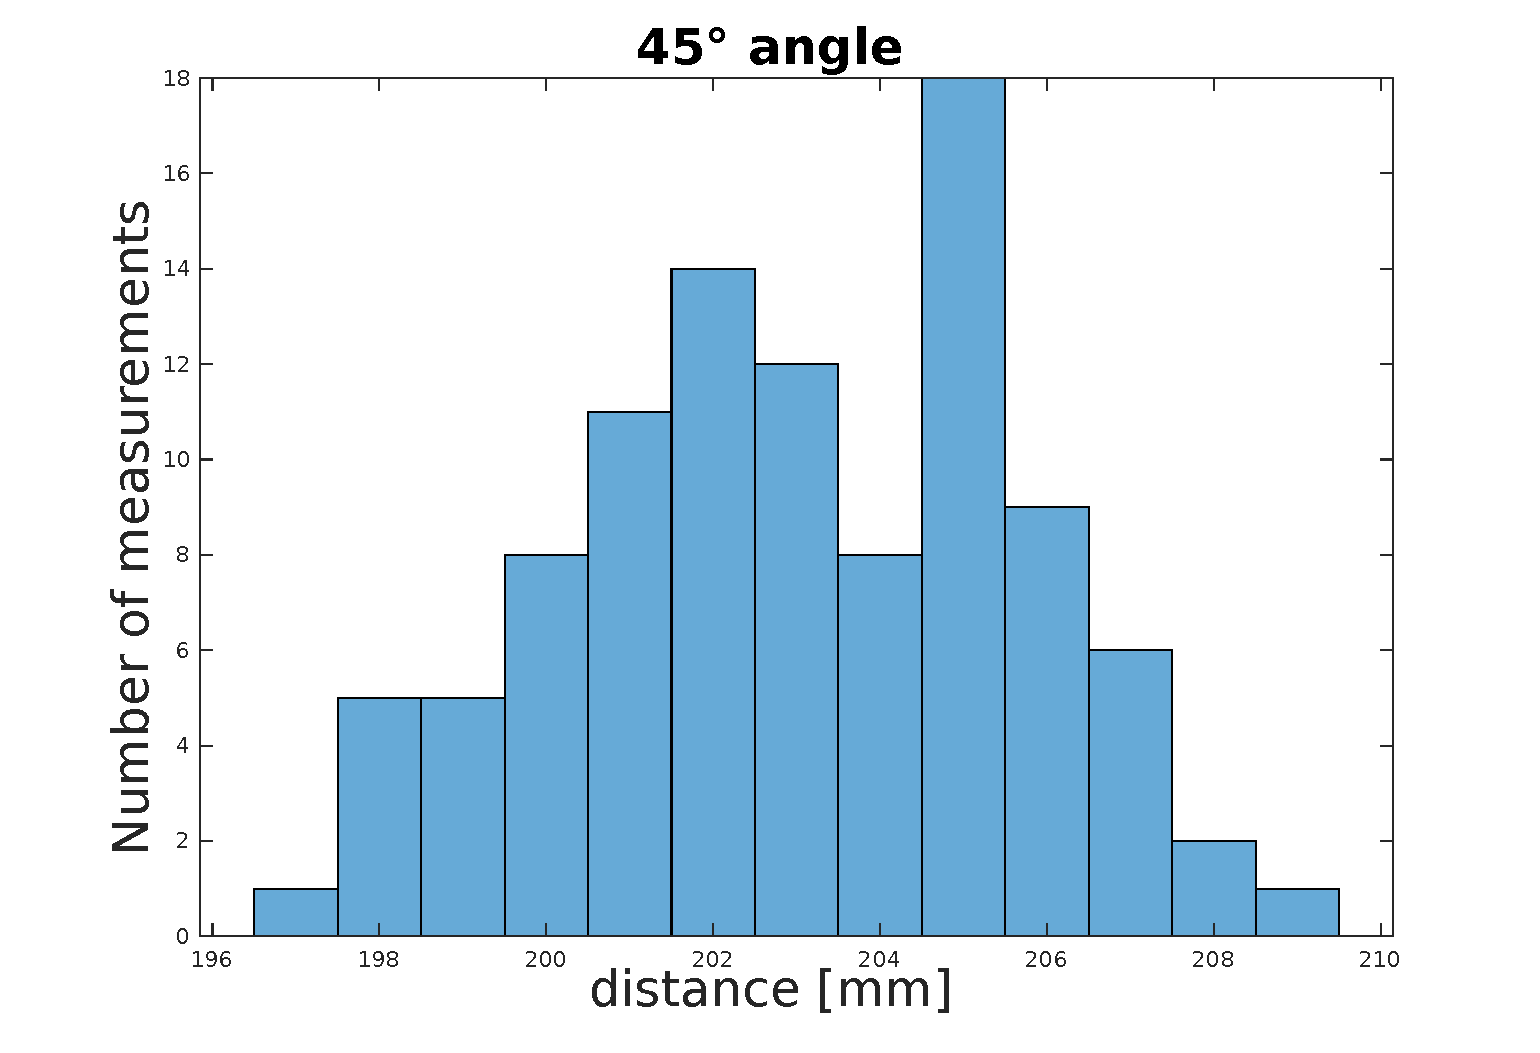
\includegraphics[width=0.9\linewidth]{pictures/plot_angles_45.pdf}
		\caption{ground truth distance $d_{truth}= \unit[20]{mm}$, Standard Error: $\sigma=\unit[2.69]{mm}$, Expected Value: $E=\unit[203.00]{mm}$, Relative angle: 45°}
		\label{fig:angle45}
	\end{minipage}
	\quad
	\begin{minipage}{0.3\textwidth}
		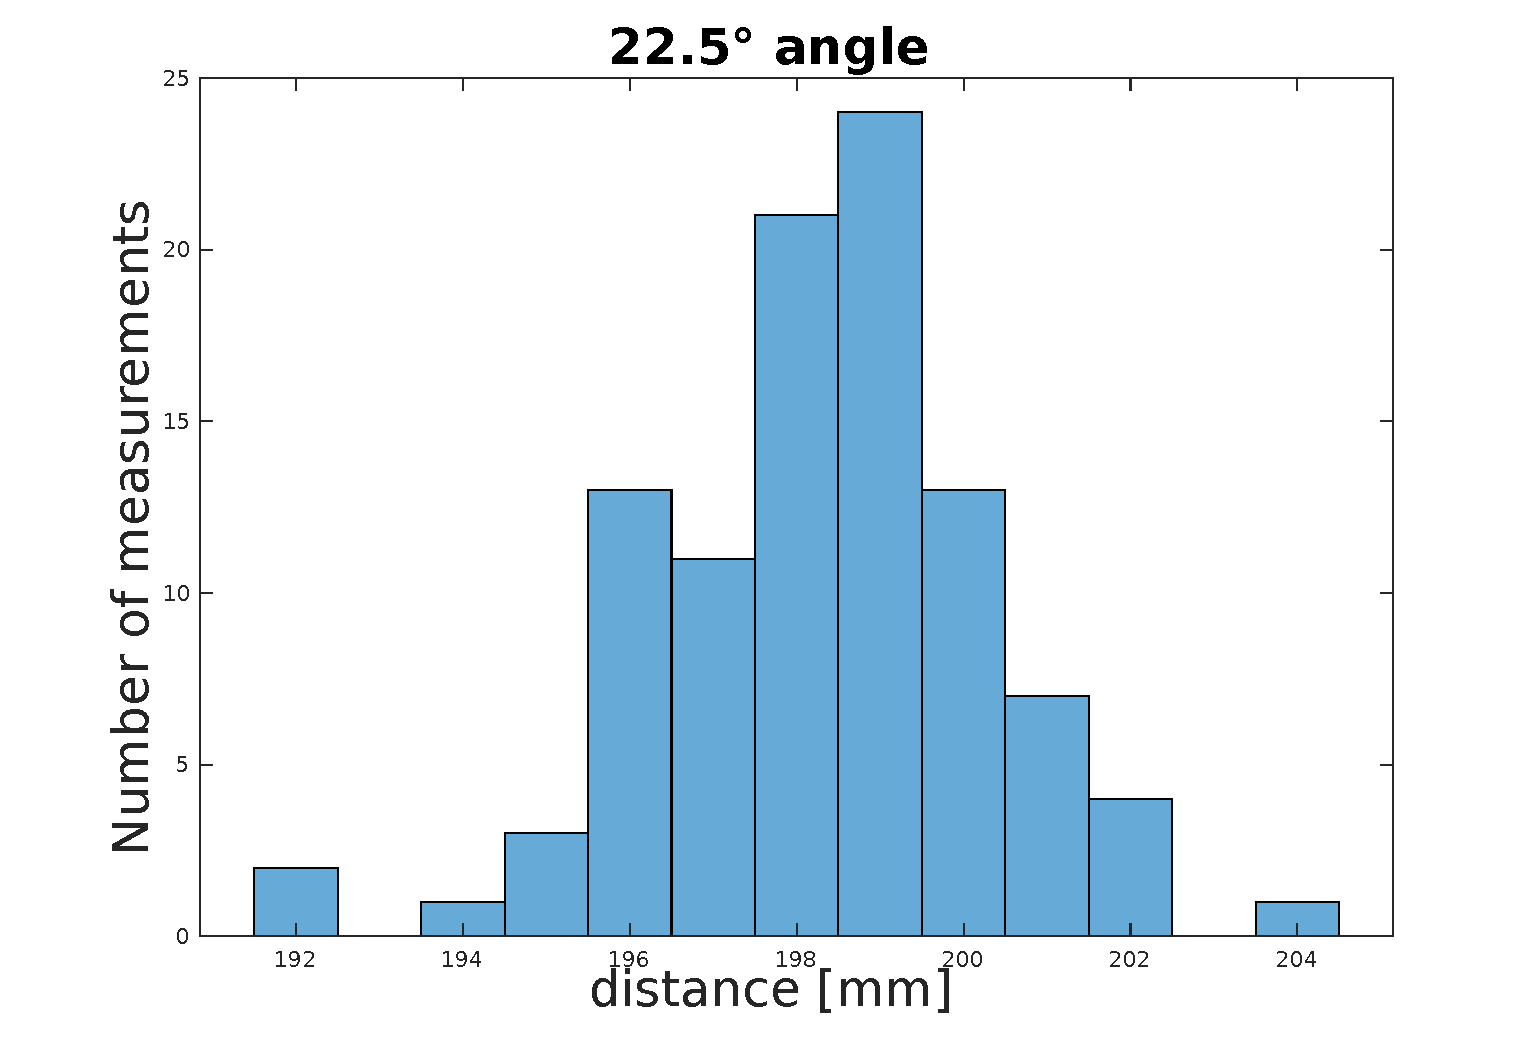
\includegraphics[width=0.9\linewidth]{pictures/plot_angles_22.pdf}
		\caption{ground truth distance $d_{truth}= \unit[20]{mm}$, Standard Error: $\sigma=\unit[3.28]{mm}$, Expected Value: $E=\unit[201.62]{mm}$, Relative angle: 22.5°}
		\label{fig:angl22.5}
	\end{minipage}
\end{figure}

A major factor of influence is IR. Outside, the slight not only decreases the accuracy, and increases the variance but moreover corrupts several measurements. With direct sunlight, up to 80\% of the measurements are corrupted (\cref{fig:meas_out}). To get reliable data, first, we filtered out the corrupted data point and, second, filtered the data with the help of the Mahalonobis distance and a Kalman filter. Filtering out the corrupted data is unproblematic, since the corrupted data point always have a value greater than 8000. For the filter, we assumed constant distance in the process model. 
\begin{equation}
	\label{eq:filter}
	\begin{split} 
	x_k & = x_{k-1} \\
	y_k & = x_k + v_k
	\end{split}
\end{equation}
The noise process $v_k$ is white, zero-mean, uncorrelated, and has known covariance matrix  $R_k$.\\
The assumption of constant distance is only valid for the evaluation of the sensor. In case of a moving sensor or target a dynamic process model has to be developed. Further, a IMU should be used for the a priori state estimate. The VL53L0X sensor fused with a IMU has a faster update rate and performs more accurate. \\

\begin{algorithm}
	\caption{Filter}\label{alg:filter}
	\begin{algorithmic}[1]
		\Procedure{FILTER}{ }
		\State $y_{data}\gets \text{raw data points}$ 
		\State Filter out corrupted data points from $y_{data}$ \\
		\textit{Initzialization:}
		\State $\hat{x}^+_0\gets\text{initial measurement }y_{data}(0)$
		\State $R_k\gets\unit[27^2]{mm^2}$ \Comment{variance of the measurements}
		\State $P^+_0\gets \unit[30]{mm^2}$ \Comment{got this value from tuning}
		\For{ each $k = (0, \text{ number of data point]}$}	
			\State  $P^-_k \gets \text{Covariance of estimation error}$
			\State	$K_k \gets \text{Kalman gains}$
		\EndFor \\
		\textit{State Estimation:}	 
		\For{ each $k = (0, \text{ number of data point]}$}
			\State \Call{Mahal}{$y_{data,k}$} \Comment{Outliers rejection with mahalanobis distance}
			\State $\hat{x}^-_k \gets \text{a priori state estimate}$
			\State $\hat{x}^+_k \gets \text{a posteriori state estimate}$
		\EndFor
		\State \Return $\hat{x}^+_k$
		\EndProcedure

	\end{algorithmic}
\end{algorithm}

By applying our filter  (\cref{alg:filter}) to the raw data points we get a convergent behavior of the data towards the ground truth distance (\cref{fig:meas_filter}).

\begin{figure}
	\centering
	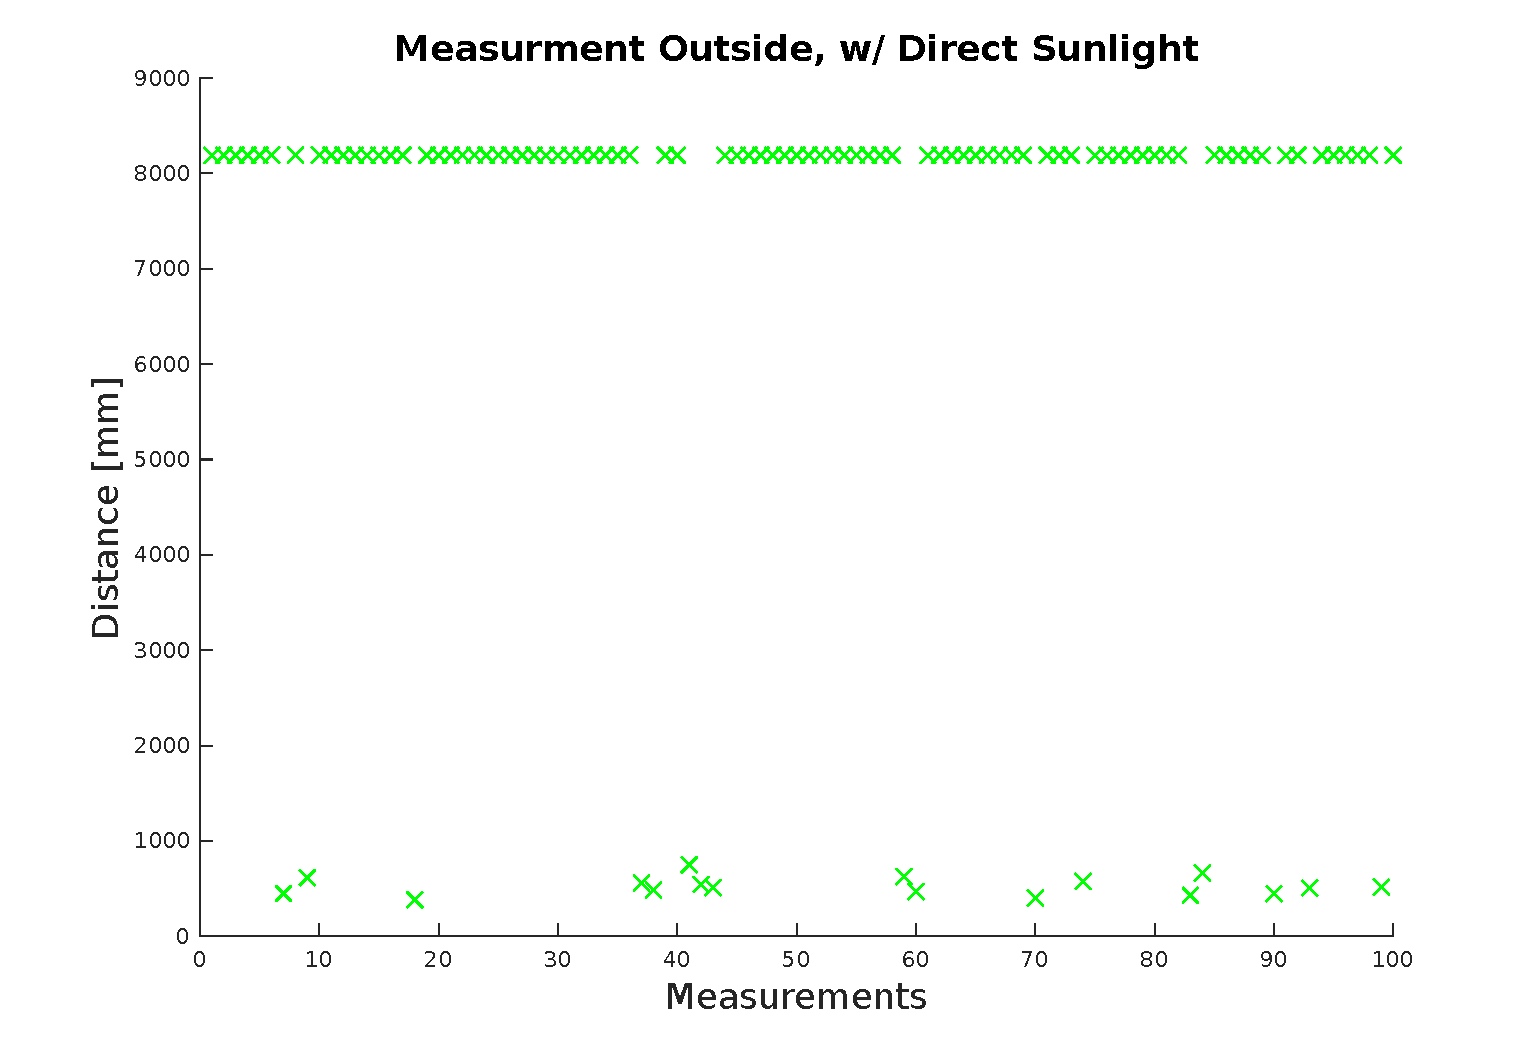
\includegraphics[width=0.9\linewidth]{pictures/plot_meas_out.pdf}
	\caption{Measurement outside with direct sunlight. All measurements above 8000 are corrupted due to the IR of the sunlight. Only 18 out of 100 measurements can be used for further processing.}
	\label{fig:meas_out}
\end{figure}


\begin{figure}
	\centering
	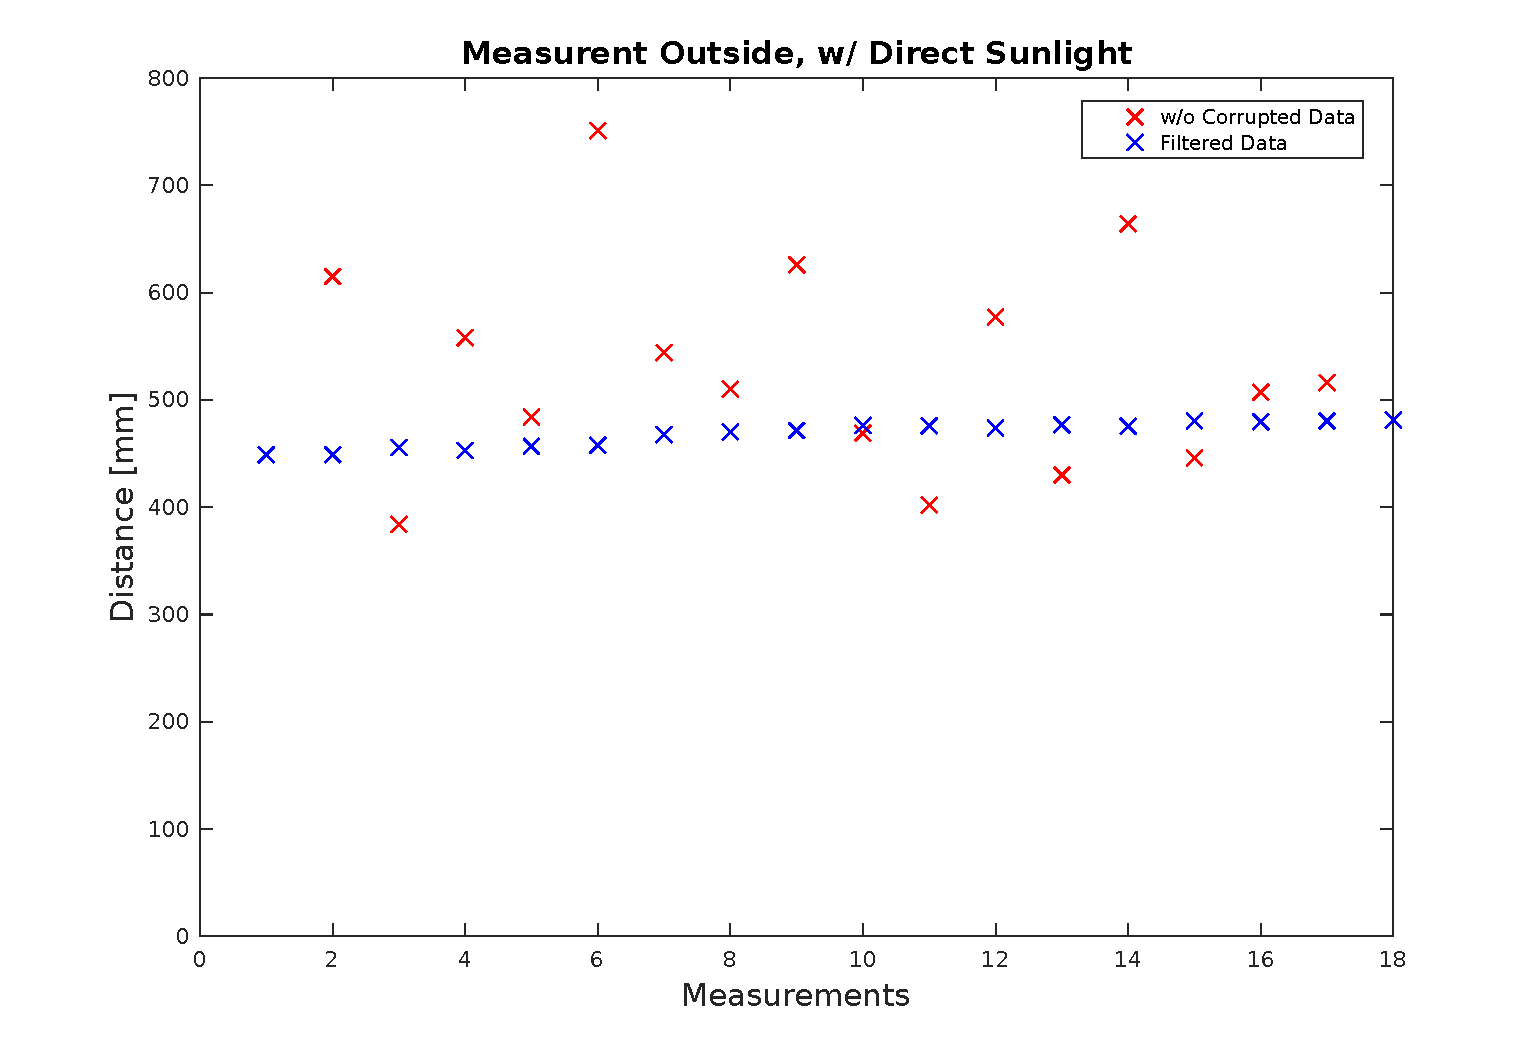
\includegraphics[width=0.9\linewidth]{pictures/plot_filter_outside.pdf}
	\caption{Data points of 100 measurement outside with direct sunlight (Corrupted data points is filtered out). Ground truth distance = \unit[500]{mm}. The raw data point (red cross) show a big variance. By applying the filter in \cref{alg:filter} we achieve an convergent behavior of the data points.}
	\label{fig:meas_filter}
\end{figure}



\subsection{Conclusion}
Without any IR source, e.g. inside, the \textit{VL53L0X ToF Ranging Sensor} operates accurate and without corrupting any data points. The variance is a few percentage and does not change significantly with increasing distance or angle relative to the target. Due to the sensor's lightweight and it's low power consumption the sensor can be adapted for the usage on a MAV, e.g. for avoidance. \\
Used with a IR source data points might get corrupted depending on the strength of the source, thus the usage of the sensor is limited. With the help of a filter, like the one presented (\cref{alg:filter}), the sensor's performance in terms of accuracy can be improved. This allows a reliable usage of the sensor. A IMU might be used for the a priori state estimate, though. \\


\section{Pixhawk}
\label{sec:pixhawk}
We use a \textit{pixhawk mRo} as a autopilot. \\
First we tried to connect four different VL53L0X sensor's to the pixhawk via I2C. Due to flash overflow due to the size of the sensor's API this wasn't possible. The calibration of the sensor requires too much computational resources.



\section{Potential Field}
\label{sec:potential field}

